\chapter{I-Mode Pedestal Stability Modeling}\label{ch:ImodeModeling}

Large, uncontrolled Edge-Localized Modes (ELMs -- see \cref{sec:hcr_elmy}) in ITER-scale operation are expected to drive unacceptable levels of pulsed heat loading and erosion damage to plasma-facing materials \cite{Loarte2003,Federici2003}.  As such, avoiding or mitigating large ELMs is a major focus of research in high-performance regimes: approaches include active ELM control in H-mode (\cref{subsec:hcr_elmy_control}) and inherently ELM-suppressed regimes (\cref{sec:hcr_elmsuppressed}).  To these we add the I-mode (\cref{sec:hcr_imode}), which appears to be naturally stable against large, deleterious ELMs in addition to its other beneficial properties (see \cref{ch:ImodePedestal}).

Confidence in plans for high-performance operation on ITER- and reactor-scale devices requires a predictive model for the pedestal structure and stability, to optimize fusion performance and ELM control or avoidance.  Recent cooperative efforts among theory, modeling, and experiment \cite{Groebner2013} have resulted in such a model for ELMy H-modes, termed EPED \cite{Snyder2009,Snyder2011}, detailed in \cref{sec:mod_eped}.  The EPED model combines constraints from peeling-ballooning MHD stability (\cref{sec:mod_pb}) \cite{Wilson2002,Snyder2004,Wilson2006}\gnote{cites?} and kinetic-ballooning turbulence (\cref{sec:mod_turbulence}) \cite{Snyder1999,Candy2005,Snyder2001}.  The EPED model has been successfully implemented in ELMy H-mode on a number of machines, including DIII-D \cite{Snyder2009,Snyder2011}, JT-60U \cite{Snyder2009}, C-Mod \cite{Walk2012}, and KSTAR \cite{Han2013}, as well as in QH-mode \cite{Snyder2012}; small/no-ELM regimes (EDA H-mode, type-II and type-III ELMy H-modes) have been shown to be stable against the drive identified in the EPED model \cite{Snyder2009}.

In this chapter, we apply the EPED approach to I-mode, examining the stability of the I-mode pedestal against peeling-ballooning MHD and kinetic-ballooning turbulence \cite{Walk2014}.  This is compared to the observed lack of large ELMs in I-mode, with a goal of examining the parameter space in which stationary ELM-free operation with I-mode is possible.  We also examine the stability and edge behavior of cases in which small, intermittent ELM-like events are observed in I-mode operation.\nicesectionending

\section{MHD Stability -- ELITE}\label{sec:imode_elite}

The triggering of large ELMs in H-mode has been identified with the interaction between pressure-driven ballooning and current-driven edge kink/peeling MHD instabilities (the latter is typically referred to as a ``peeling'' mode to distinguish it from similarly current-driven core kink modes) in the pedestal \cite{Wilson2002,Snyder2004,Wilson2006}.  Numerical studies of these instabilities using the ELITE code \cite{Wilson2002,Snyder2003}, detailed in \cref{subsec:mod_elite}, have proven quite successful in capturing the physics of the ELM trigger.

\subsection{ELITE Implementation}\label{subsec:imode_elite_setup}

At its simplest, a single pass in ELITE calculates the growth rate of the peeling-ballooning instability at fixed toroidal mode number $n$ for a given plasma profile (to wit, the pressure gradient and current density in the pedestal) and equilibrium \cite{Snyder2013}\gnote{how much of this in ch 3?}.  This requires a reconstructed magnetic equilibrium with sufficiently high point density to capture the rapid variation in flux surfaces near the edge -- all results in this chapter were prepared using high-resolution EFIT \cite{Lao1985} reconstructions constrained by kinetic profiles\gnote{better ref for kinetic EFIT?} -- and high-resolution diagnostics to generate accurate profile measurements in the pedestal.  To fully capture the physics of the pedestal, however, it is beneficial to visualize the pedestal relative to the full stability boundary (see \cref{fig:mod_pbcartoon} for a schematic illustration), typically expressed in terms of the pressure-gradient and current-density drive terms.  

Beginning from the experimental result, the profiles are scaled at fixed pedestal width, such that the pressure pedestal height or peak current density is increased or decreased relative to the original by a scalar factor, after which a self-consistent EFIT reconstruction is attempted.  This effectively fills in a grid in $\alpha_{MHD} - j$ space.  Horizontal slices scaling the pressure pedestal height (and therefore gradient) at fixed current, and vertical slices scaling the current density at fixed $\nabla p$ -- although ELITE does not explicitly distinguish between density and temperature profiles, these slices implicitly vary density and temperature relative to each other (for example, increased bootstrap current at fixed $\nabla p$ in a vertical slice requires increased density and decreased temperature, and vice versa for horizontal slices) \cite{Snyder2013}.  Note that the practice described in \cref{sec:mod_eped} of increasing pressure (and pressure gradient) at fixed width to find the maximum ELM-stable pressure as a function of width is essentially a diagonal slice through the grid: only the pressure profile is explicitly scaled, with the bootstrap current allowed to self-consistently vary\gnote{cite?}, and will increase with increasing $\nabla p$.  At each point in the $\alpha_{MHD} - j$ grid, ELITE is run on a range of mode numbers (here $5 \le n \le 35$) to find the most unstable mode\gnote{note low-$n$ peeling, higher-$n$ ballooning in ch 3} and its growth rate; this is normalized to diamagnetic stabilization effects by the threshold for instability onset, $\gamma_{MHD} > \omega_{*eff}/2$ where $\omega_{*eff}$ is the effective diamagnetic frequency accounting for variation in the pedestal, as implemented in EPED1.6 (see \cref{subsec:mod_eped16}).

\begin{figure}[p]
 \pushtooutside
 \ffigbox[\FBwidth]{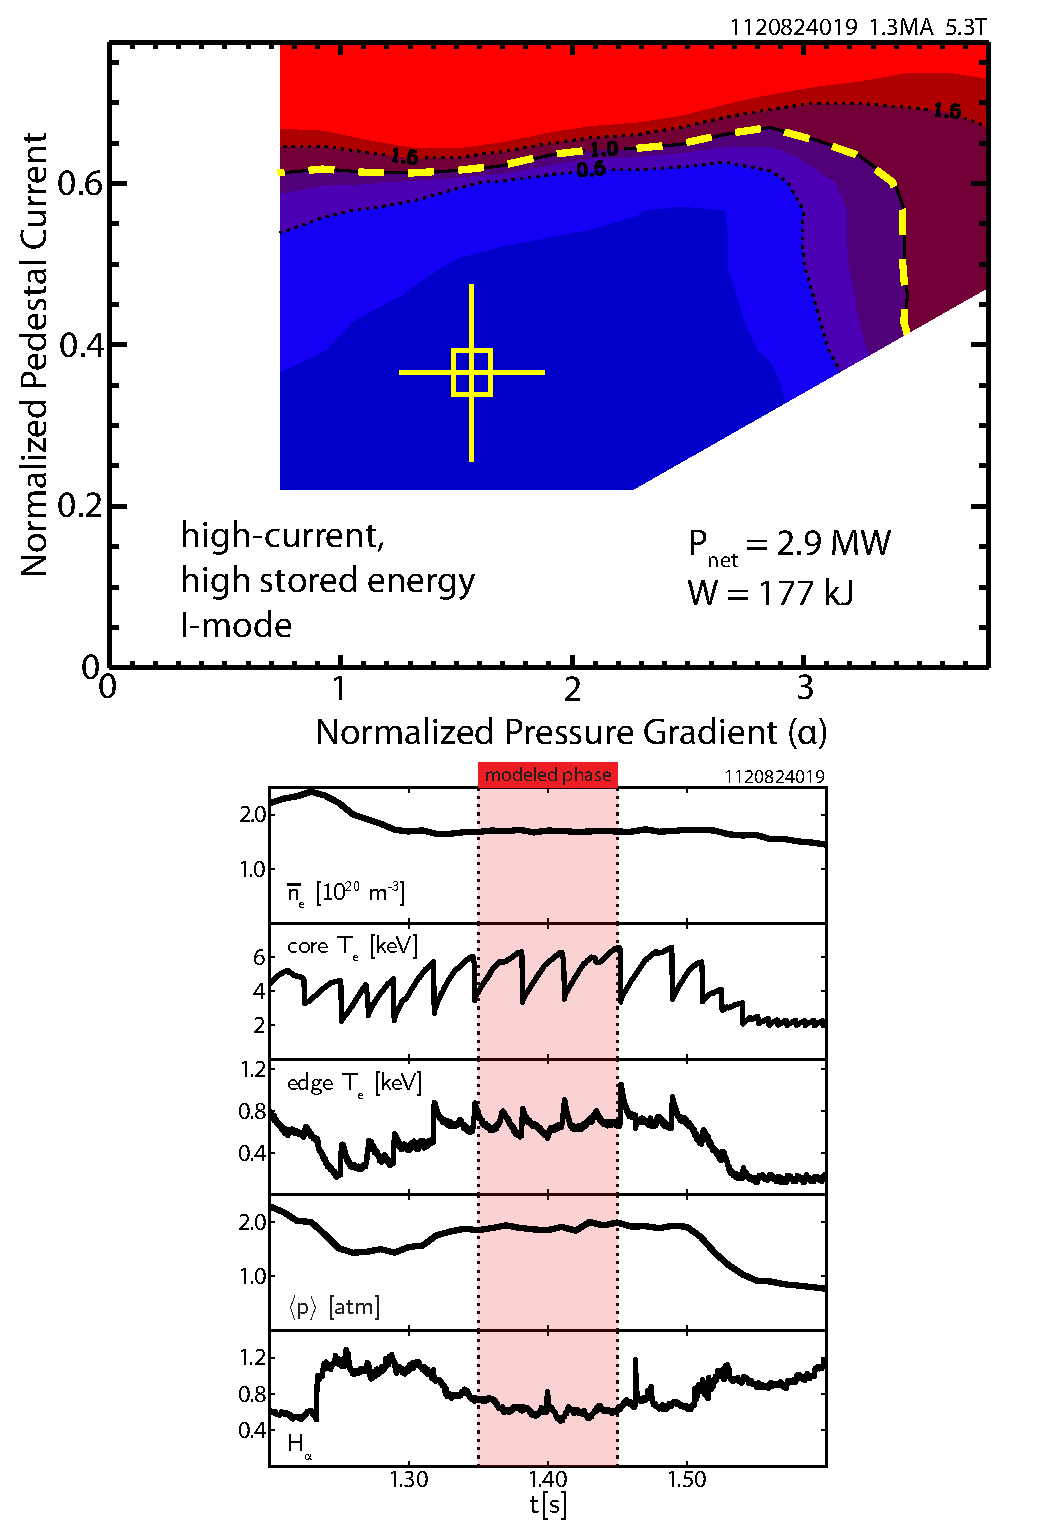
\includegraphics[width=150mm]{graphics/IModeModeling/1120824019_ELITE_stitch_vert.pdf}}{\caption[I-mode pedestal MHD stability contour generated by ELITE.]{MHD stability contour for a high-current ($\SI{1.3}{\mega\ampere}$), high-performance I-mode generated by the ELITE code.  The experimental measurement is shown by the crosshair, with the stability boundary indicated by the yellow dashed line.  Parameters for the modeled phase of the discharge are shown below.  The I-mode pedestal is observed to be far from both the peeling and ballooning MHD stability boundaries.}\label{fig:imode_elite_noelm}}
\end{figure}

\subsection{I-Mode ELITE Calculations}\label{subsec:imode_elite_calc}

An ELITE calculation for the I-mode pedestal is shown in \cref{fig:imode_elite_noelm}, along with parameters (line-averaged density, core and edge $T_e$, global-average pressure, and $H_\alpha$ emission) for the modeled phase of the discharge.  The pedestal, indicated by the yellow crosshair, is far from both the peeling and ballooning MHD stability boundaries calculated by ELITE (indicated by the yellow dashed line, marking the $\gamma/(\omega_{*eff}/2) = 1$ contour).  This is consistent with the observed lack of large ELMs, even in higher-performance I-modes (both in the normalized sense, with $H_{98} = 1.02$ and $\beta_N = 1.0$, and in absolute terms, $W_{MHD} = \SI{177}{\kilo\joule}$ in the case in \cref{fig:imode_elite_noelm}).  The calculated MHD stability is intuitively understood from the I-mode pedestal profile: the lack of a strong density pedestal reduces both the total pressure gradient, reducing the ballooning drive, and the edge current, reducing the peeling drive (recall from \cref{eq:jboot} that $\nabla n_e$ is the dominant term setting the bootstrap current).  A comparison of the pedestal profiles, with pressure gradient and edge current density, between I-mode and H-mode is shown in \note{ref to figure}:

\noindent \note{$\nabla p$, bootstrap graphic here!}

Although I-mode is free of the regular, large ELMs typical of (type-I) ELMy H-mode, under certain conditions -- particularly reduced toroidal field and plasma current -- small ($<1\%$ drop in stored energy) intermittent ELM-like events are occasionally observed in I-mode.  However, when examined in ELITE (\cref{fig:imode_elite_stelm}) these cases are found to still be far from the peeling-ballooning boundary.  These intermittent events occur in conjunction to sawtooth heat pulses reaching the edge, visible on the fast ECE $T_e$ signal, indicating that the events are potentially triggered by transient modification of the pedestal by the heat pulse -- however, these events are not consistently triggered on each sawtooth crash under similar conditions.  More study is required on this front, with initial results shown in \cref{sec:imode_elms}.

\begin{figure}[p]
 \pushtooutside
 \ffigbox[\FBwidth]{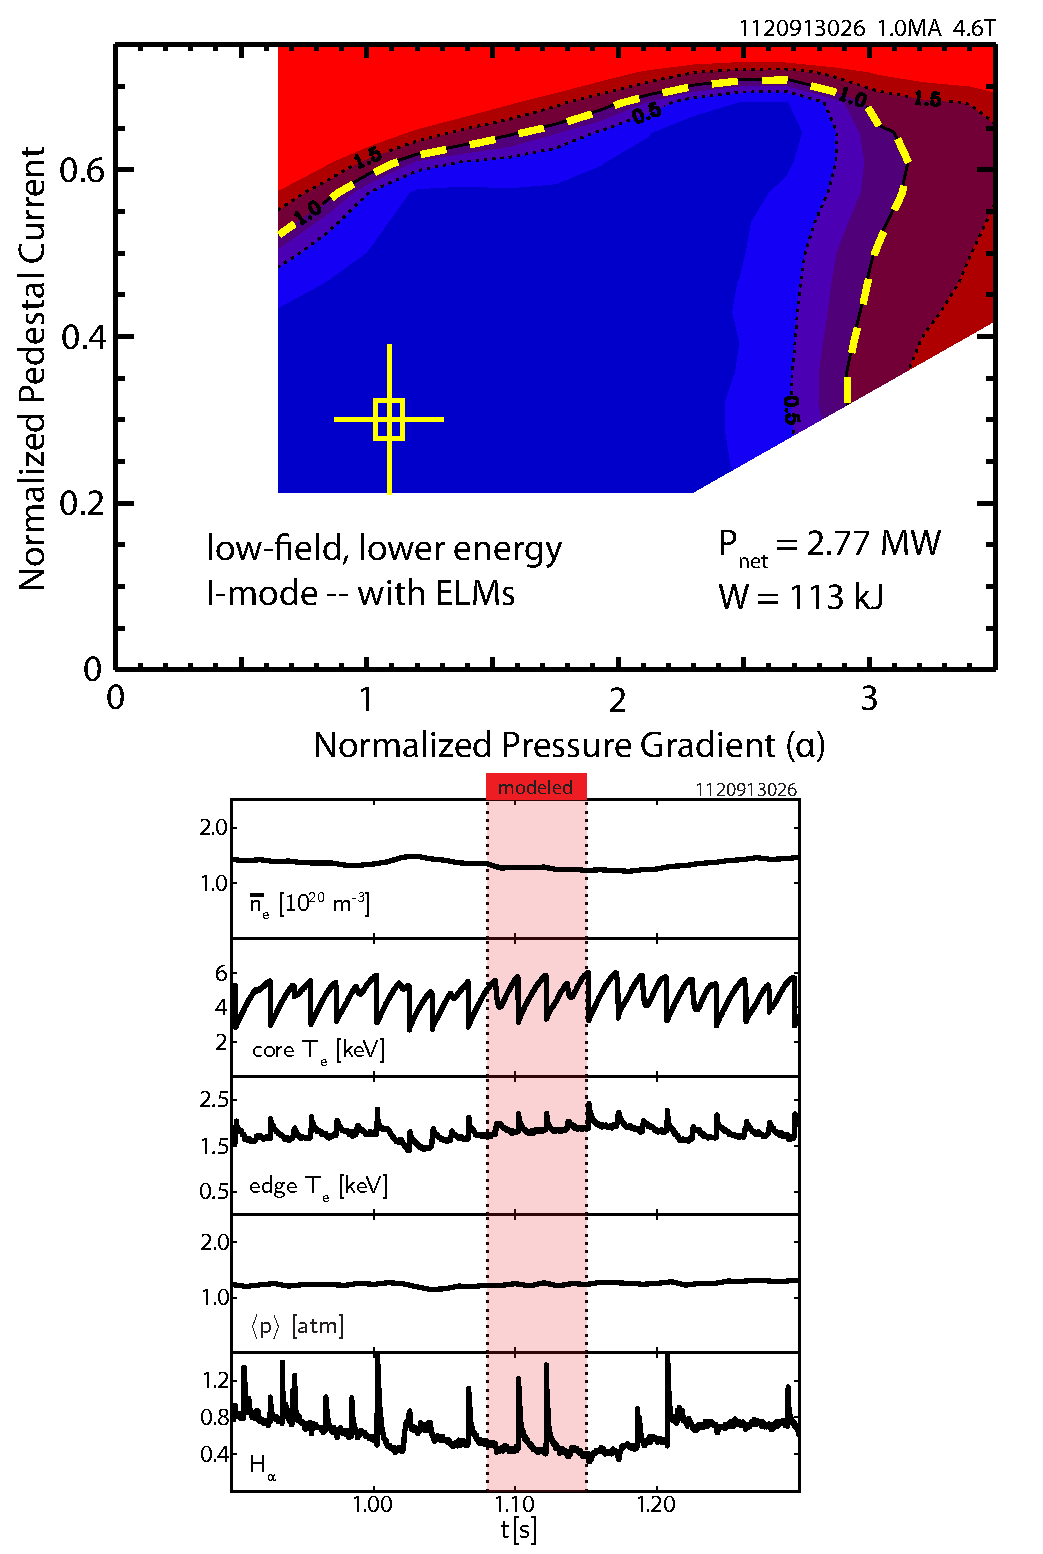
\includegraphics[width=150mm]{graphics/IModeModeling/1120913026_ELITE_stitch_vert.pdf}}{\caption[I-mode pedestal MHD stability contour generated by ELITE -- low-field case exhibiting ELM-like events.]{MHD stability contour for a low-field, lower-energy I-mode generated by the ELITE code.  The experimental measurement is shown by the crosshair, with the stability boundary indicated by the yellow dashed line.  Parameters for the modeled phase of the discharge are shown below.  This case exhibited small,intermittent ELM-like events, but is still calculated to be peeling-ballooning stable.}\label{fig:imode_elite_stelm}}
\end{figure}



\begin{figure}
 \pushtooutside
 \ffigbox[\FBwidth]{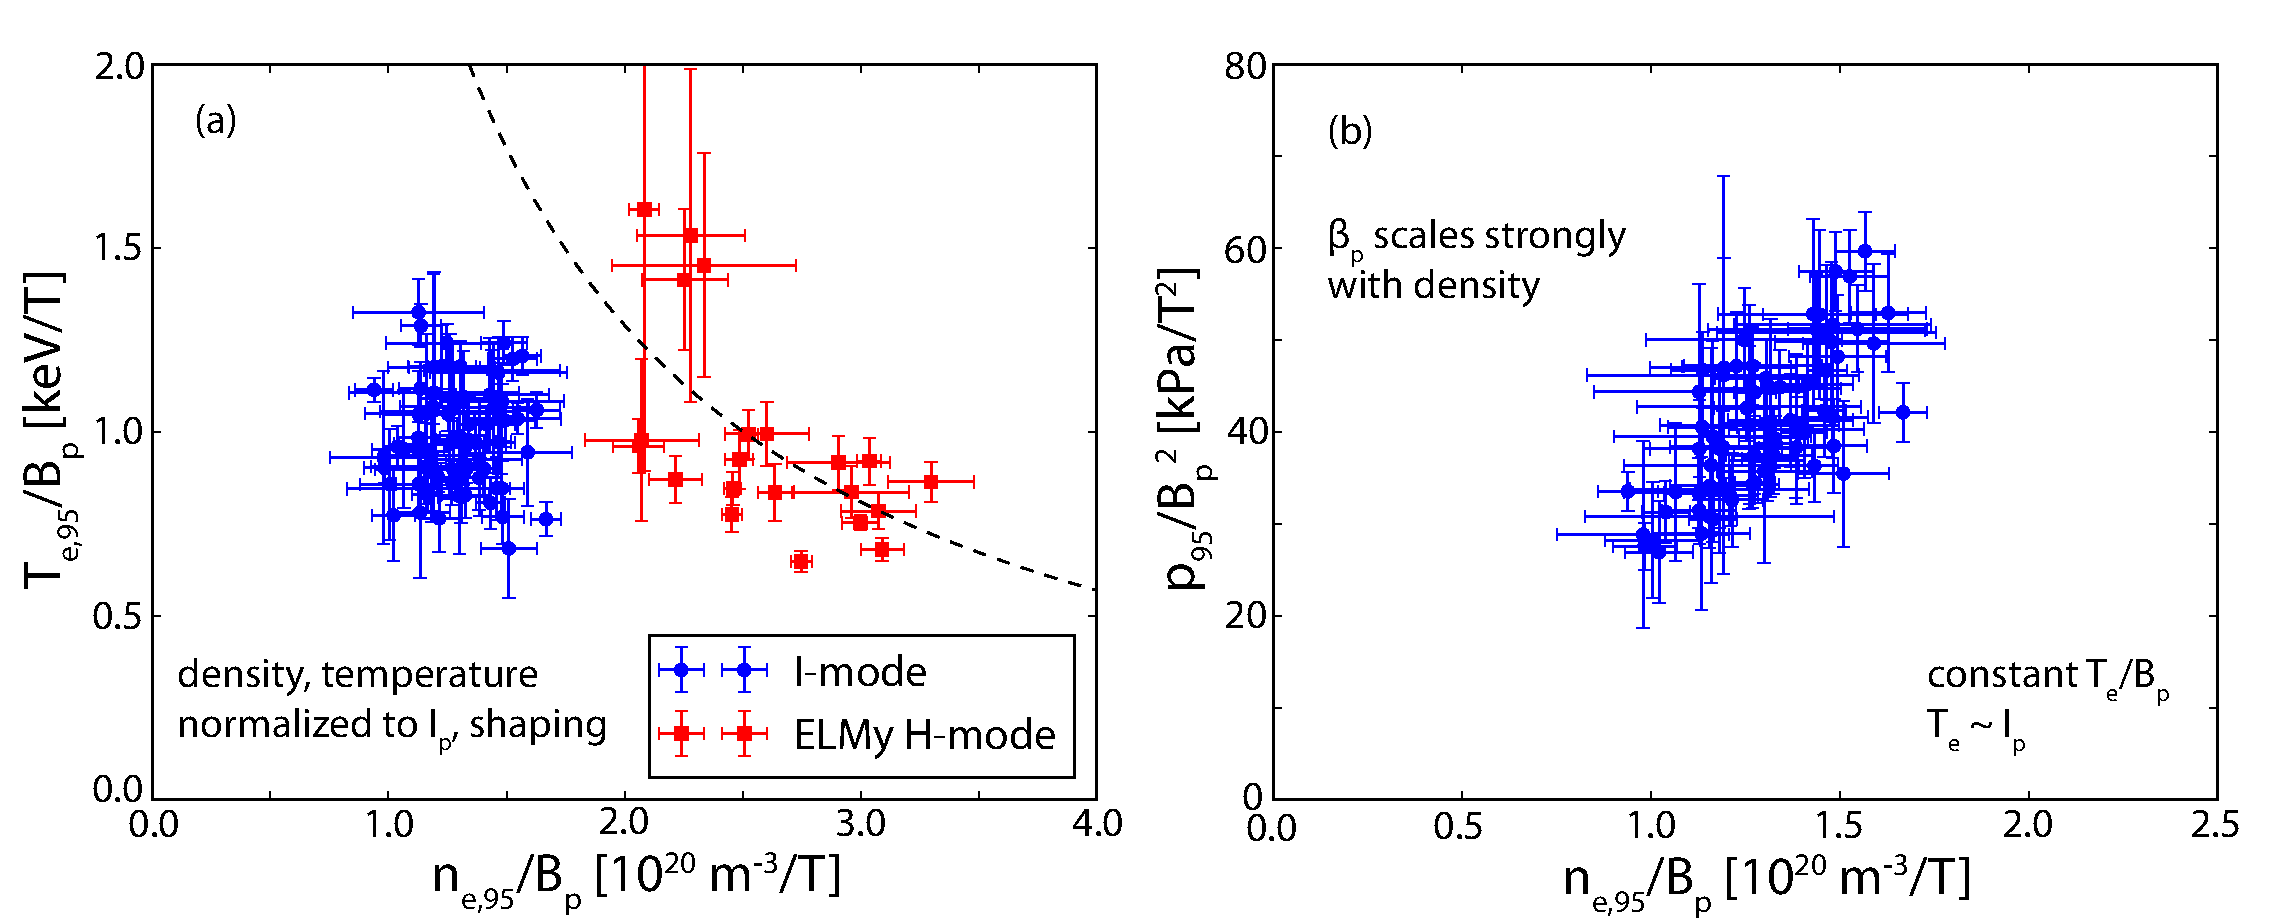
\includegraphics[width=150mm]{graphics/IModeModeling/neBp_stitch.pdf}}{\caption[Normalized pedestal temperature and pressure versus density.]{Pedestal temperature (left) and pressure (right) versus pedestal density.  Parameters are normalized to the edge poloidal field -- this accounts for plasma-current variation in the datapoints, as well as allowing a natural representation of MHD boundaries.  (a) Pedestal temperature vs. density for I-mode and ELMy H-mode.  Due to the poloidal-field normalization, hyperbolae in the parameter space are curves of constant $\beta_{p,ped}$.  ELMy H-modes lie, to lowest-order approximation, on a $\beta_{p,ped}$-limited curve (indicated by the dashed line) with the expected inverse relationship between density and temperature; I-mode $n_e$ and $T_e$, however, are uncorrelated.  (b) Normalized pedestal pressure versus density in I-mode.  Pedestal poloidal beta trends linearly with (normalized) density, rather than lying on the $\beta_{p,ped}$-limited line expected for MHD-limited pedestals, consistent with the strong response of the I-mode pedestal to fueling (see \cref{subsec:imode_fueling}).  I-mode data lie on a line of constant $T_e/B_p$, consistent with the observed $T_{e,ped} \sim I_p$ seen in \cref{subsec:imode_temp}.}\label{fig:neBp_stitch}}
\end{figure}

\nicesectionending

\section{KBM and Infinite-$n$ MHD Stability}\label{sec:imode_baloo}

\begin{figure}
 \pushtooutside
 \ffigbox[\FBwidth]{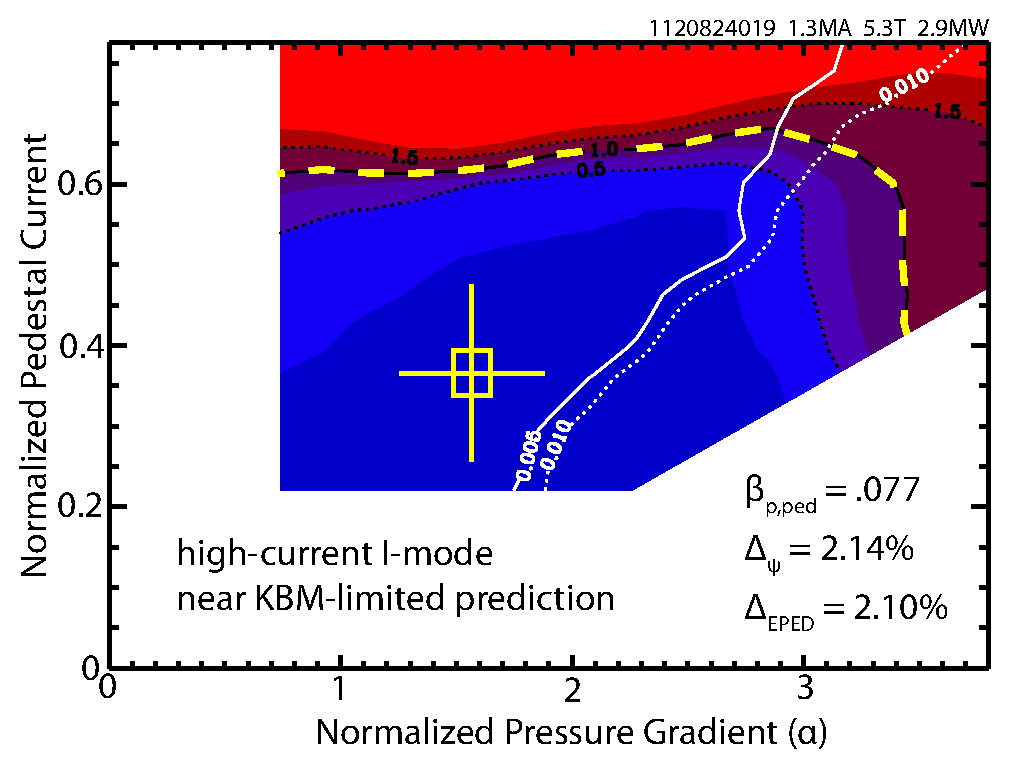
\includegraphics[width=150mm]{graphics/IModeModeling/1120824019_1400n5_35_gamws16_bal.pdf}}{\caption[]{}\label{fig:imode_baloo_noelm}}
\end{figure}

\begin{figure}
 \pushtooutside
 \ffigbox[\FBwidth]{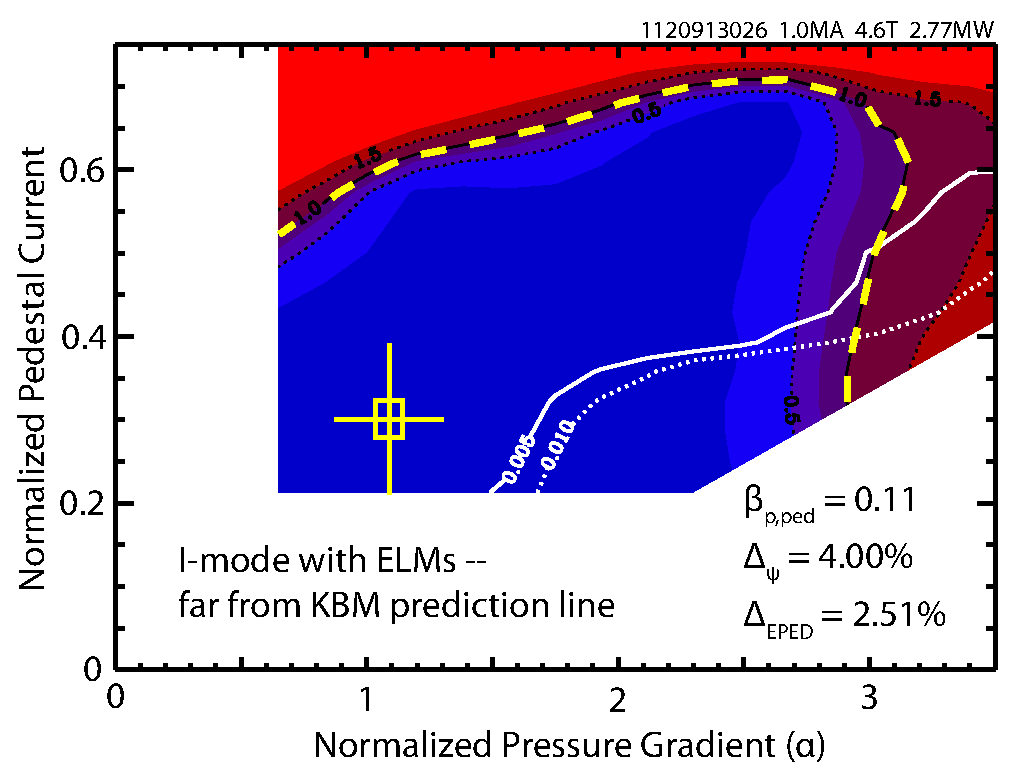
\includegraphics[width=150mm]{graphics/IModeModeling/1120913026_1186n5_35_bal_jalpha.pdf}}{\caption[]{}\label{fig:imode_baloo_stelm}}
\end{figure}

\nicesectionending

\section{Intermittent ELMs in I-Mode}\label{sec:imode_elms}

\begin{figure}
 \pushtooutside
 \ffigbox[\FBwidth]{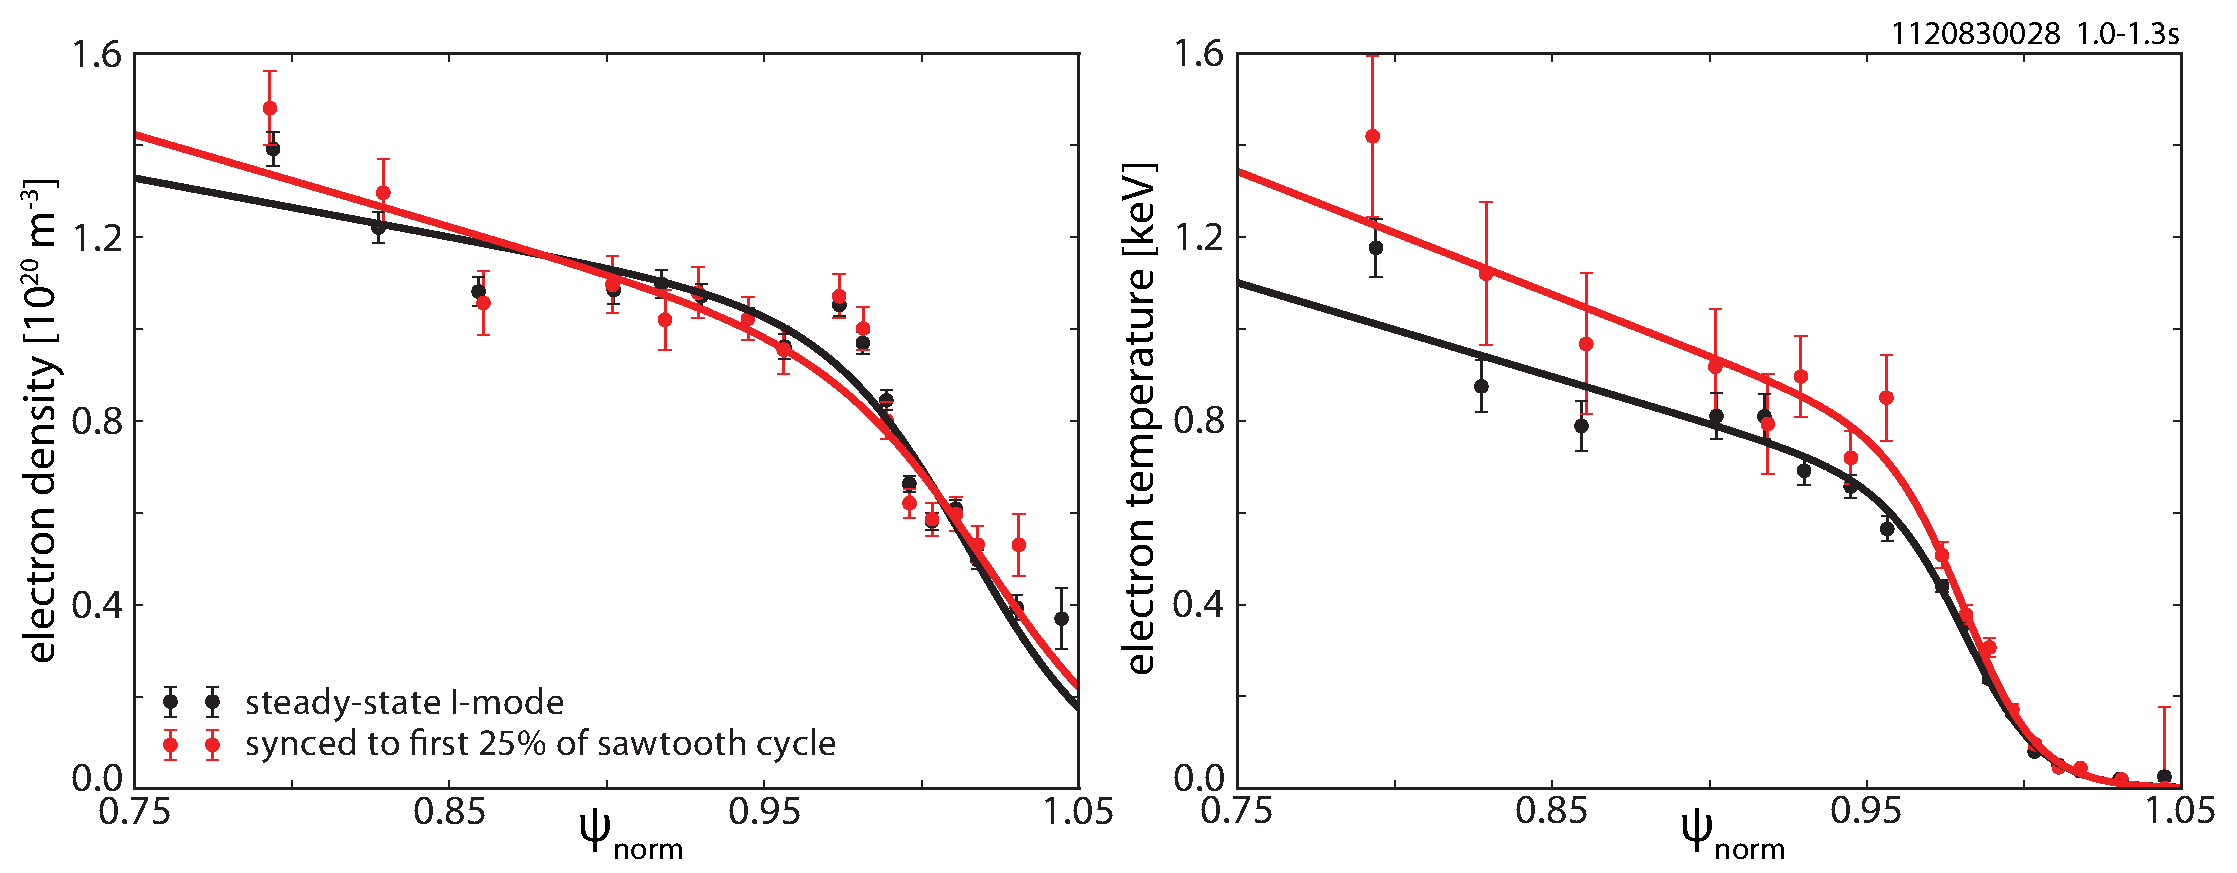
\includegraphics[width=150mm]{graphics/IModeModeling/1120830028_prof_stbin.pdf}}{\caption[]{}\label{fig:prof_stbin}}
\end{figure}

\begin{figure}
 \pushtooutside
 \ffigbox[\FBwidth]{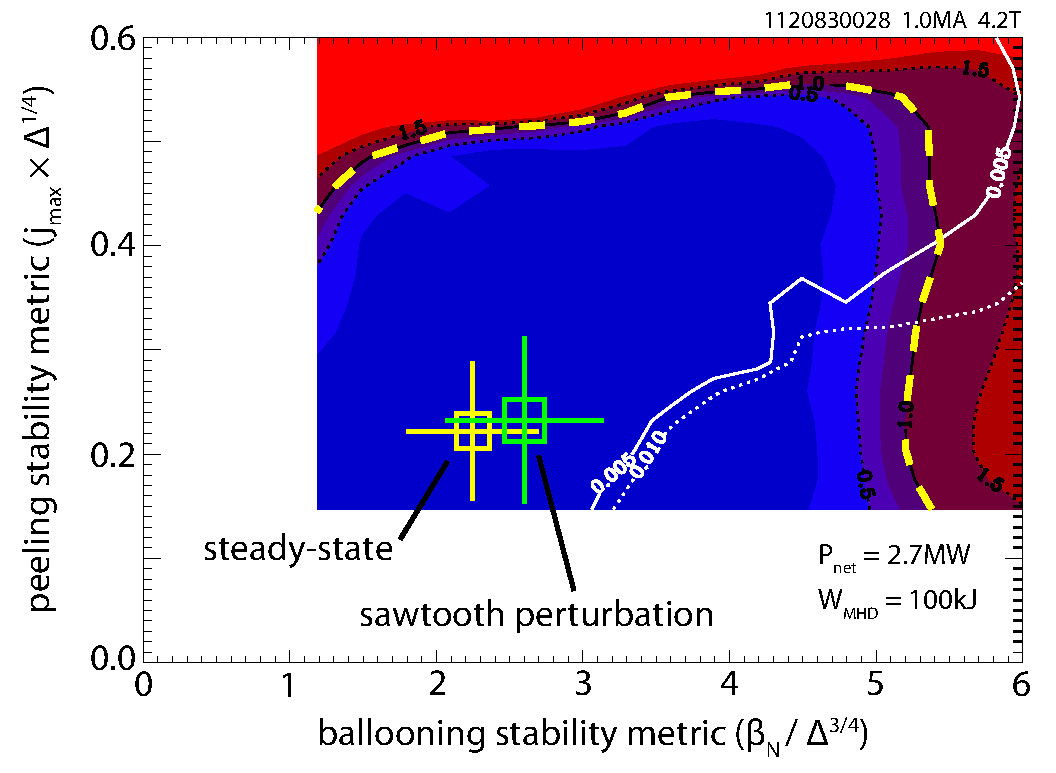
\includegraphics[width=150mm]{graphics/IModeModeling/1120830028_stbin_elite.pdf}}{\caption[]{}\label{fig:imode_stbin}}
\end{figure}

\begin{figure}
 \pushtooutside
 \ffigbox[\FBwidth]{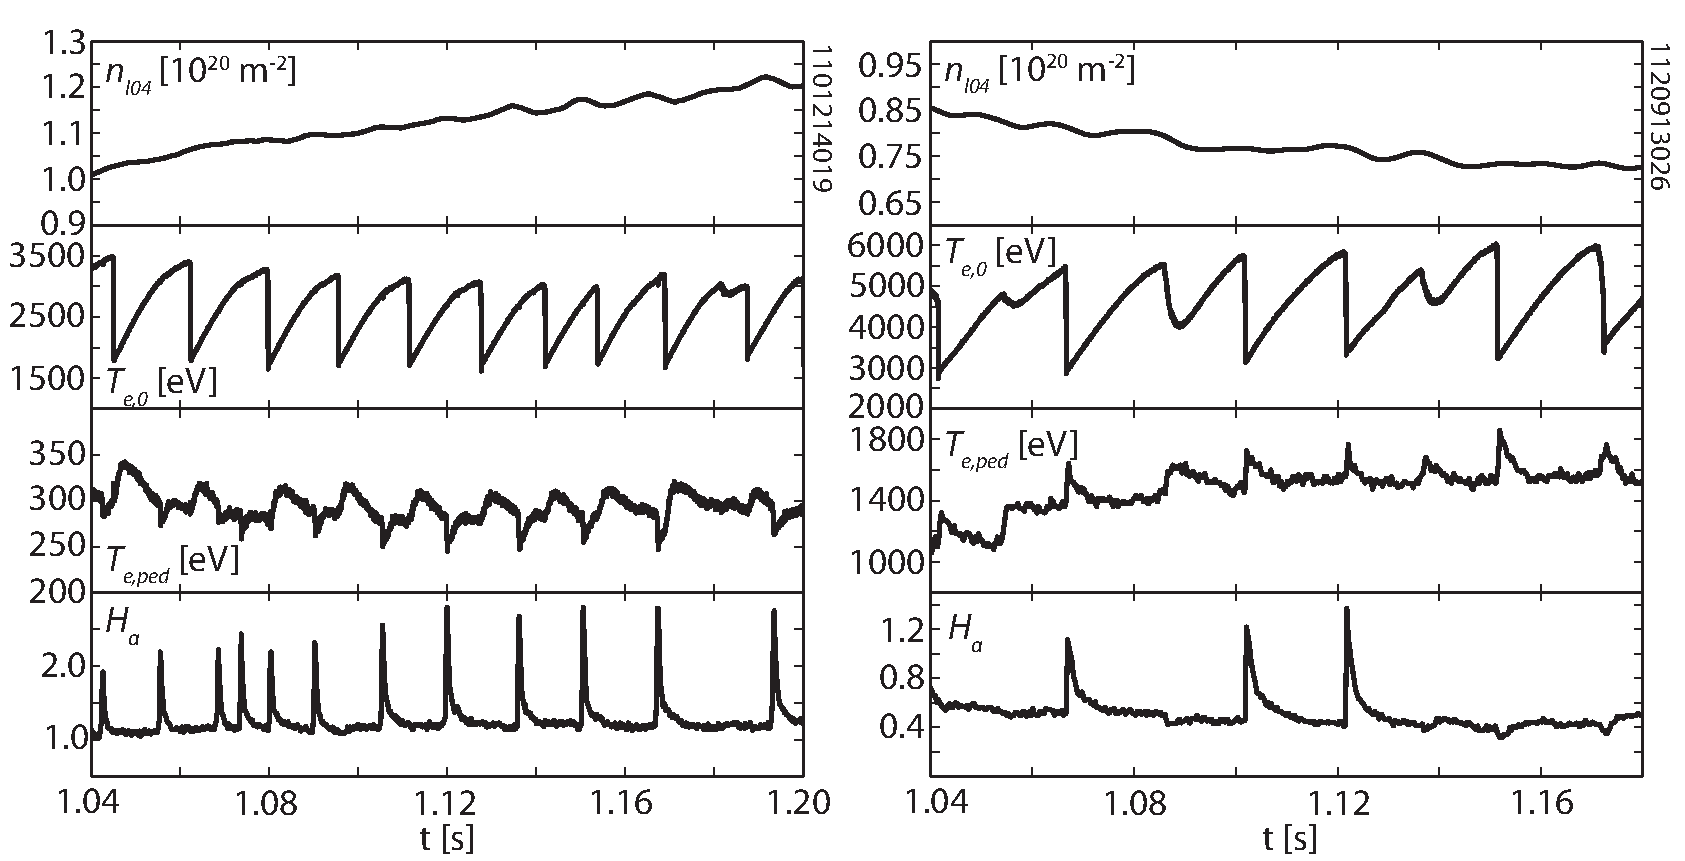
\includegraphics[width=150mm]{graphics/IModeModeling/trace_elmy_imode.pdf}}{\caption[]{}\label{fig:trace_elmy_imode}}
\end{figure}

\begin{figure}
 \pushtooutside
 \fcapside[60mm]{\caption[]{}\label{fig:trace_imode_welms}}{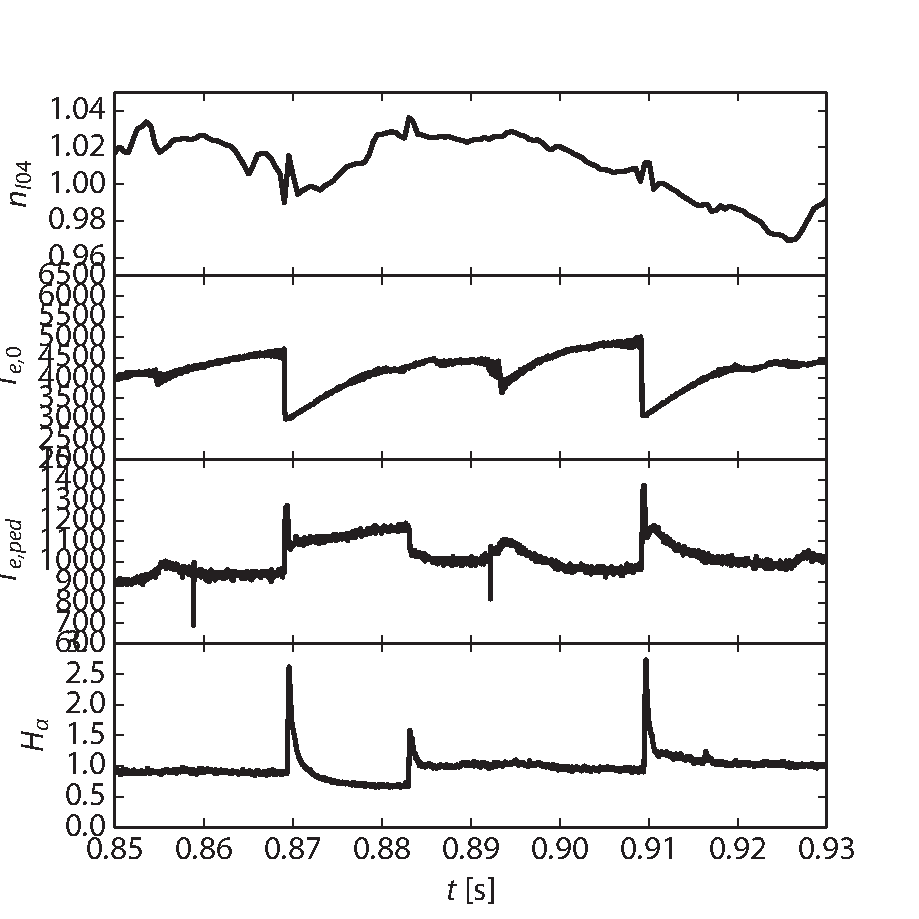
\includegraphics[width=100mm]{graphics/IModeModeling/trace_imode_welms_2.pdf}}
\end{figure}

\begin{figure}[p]
 \pushtooutside
 \ffigbox[\FBwidth]{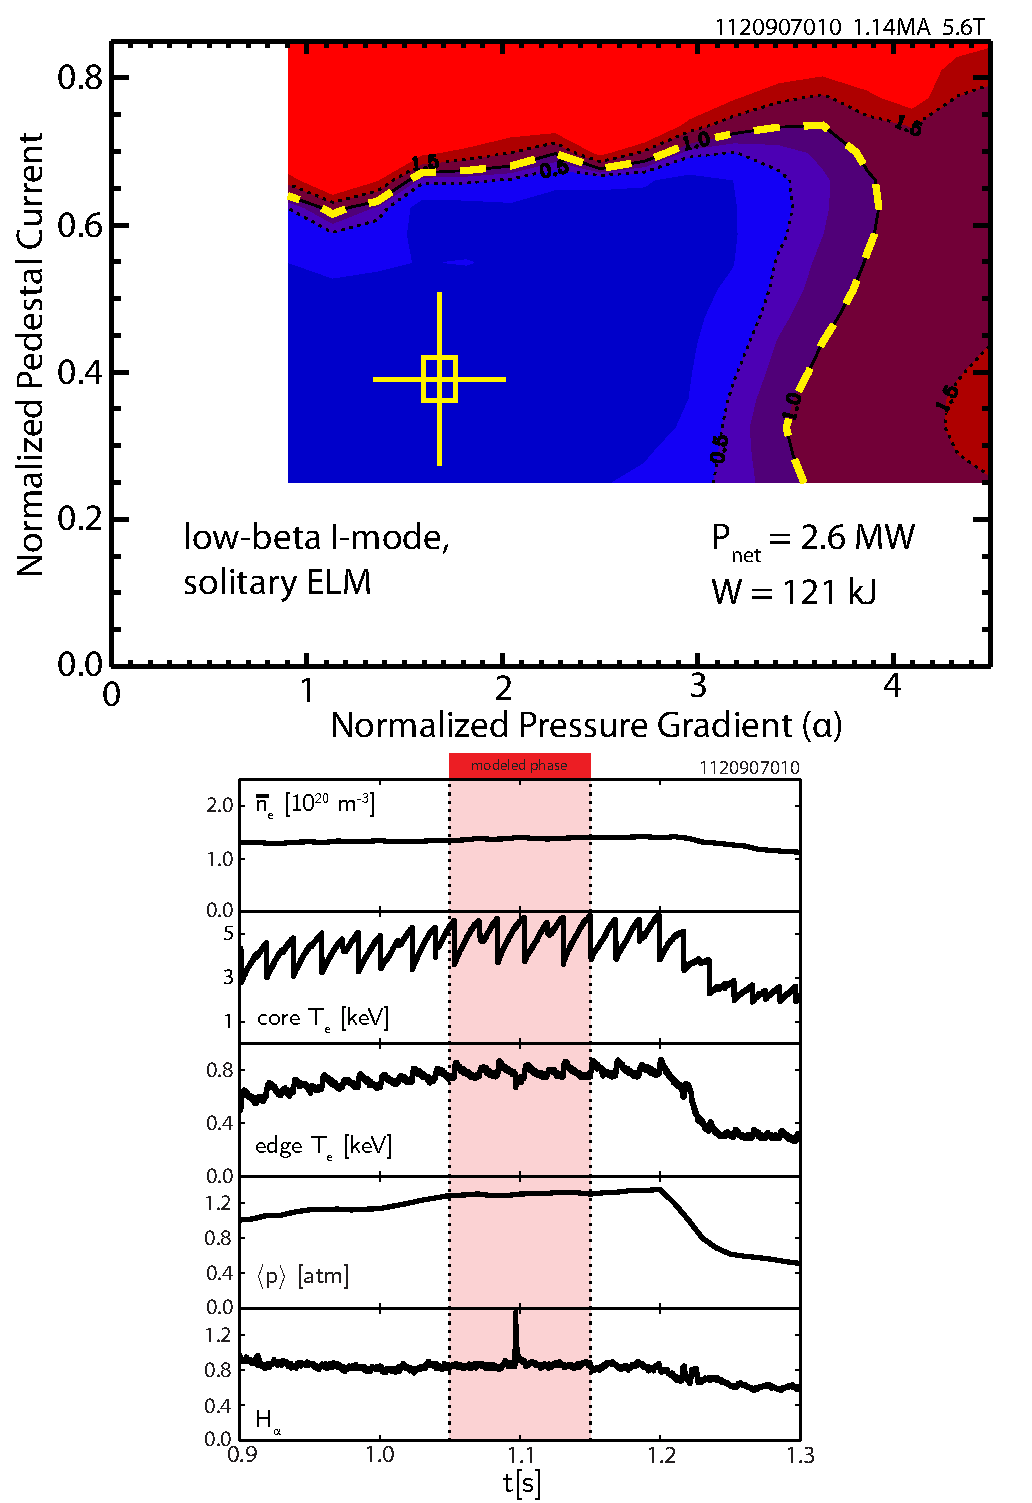
\includegraphics[width=150mm]{graphics/IModeModeling/1120907010_ELITE_stitch_vert.pdf}}{\caption[]{}\label{fig:imode_elite_nonstelms}}
\end{figure}

\begin{figure}
 \pushtooutside
 \ffigbox[\FBwidth]{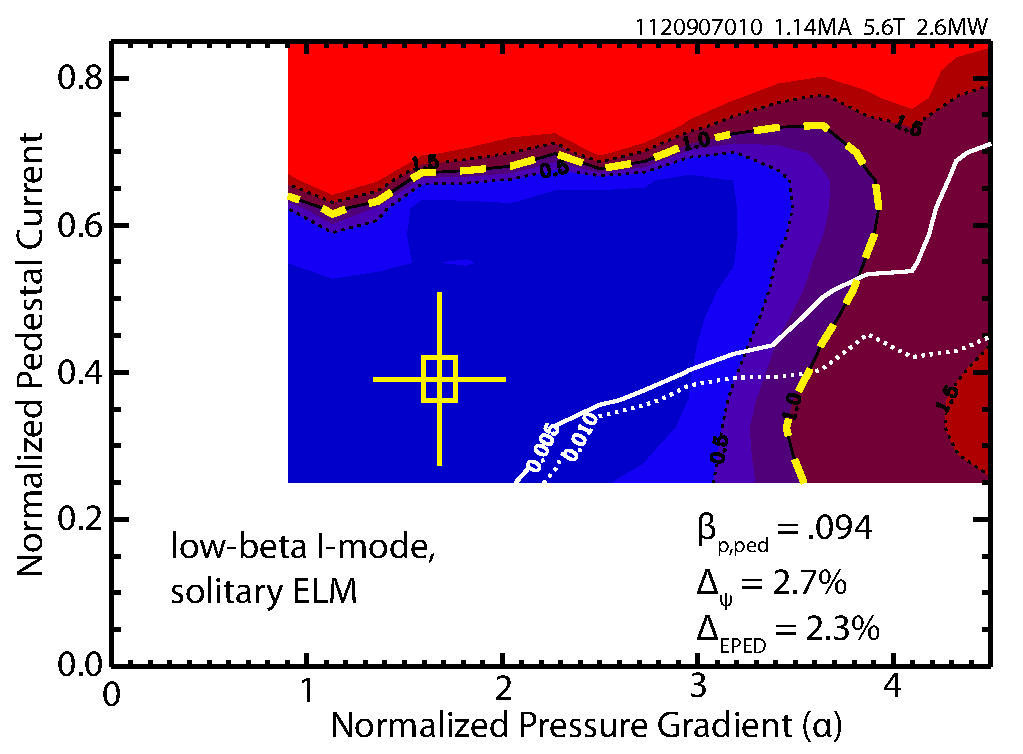
\includegraphics[width=150mm]{graphics/IModeModeling/1120907010_1100n5_35_gamws16_bal.pdf}}{\caption[]{}\label{fig:imode_baloo_nonstelms}}
\end{figure}

\nicechapterending

\bibliographystyle{../plainurl}
\bibliography{../references}